\documentclass[a4j,12pt,]{jarticle}
 \usepackage{float}
 \usepackage{siunitx} %%SI単位系用
 \usepackage{amssymb, amsmath}
 \usepackage{ascmac,here,txfonts}
 \usepackage{hyperref}
 \usepackage{listings}
 \usepackage{pxjahyper}
 \usepackage[dvipdfmx]{graphicx}
 \usepackage{amssymb, amsmath}
  \usepackage{listings}
  \usepackage[dvipdfmx]{color}
 
 \lstset{
   language={Python},
   basicstyle={\ttfamily},
   identifierstyle={\small},
   commentstyle={\small\itshape},
   keywordstyle={\small\bfseries},
   ndkeywordstyle={\small},
   stringstyle={\small\ttfamily},
   frame={single},
   breaklines=true,
   columns=[l]{fullflexible},
   numbers=left,
   xrightmargin=0zw,
   xleftmargin=3zw,
   numberstyle={\scriptsize},
   stepnumber=1,
   numbersep=1zw,
   lineskip=-0.5ex,
 }
\begin{document}

{\noindent\small 第16回報告書 \hfill\today}
\begin{center}
  {\Large ElasticSearchサーバーのデータ移行について}
\end{center}
\begin{flushright}
  祖父江匠真 \\
\end{flushright}

\section{概要}
今回は, 133.71.201.197から133.71.106.141へのElasticSearchサーバー間のリサイクル館の太陽光パネルの測定データ移行とkibanaを用いた可視化結果について報告する.
また, 133.71.106.168のElasticSearchサーバーにあったmovement\_diaryインデックスとmovement\_diary01インデックスのドキュメントについて調査した結果も報告する.

\section{データ移行手順について}

データ移行を行う上で, ローカルマシンにJSON形式でダンプしていたデータと, 133.71.201.197のElasticSearchサーバー上に存在するデータとの間で重複しているデータが一部存在しており, この重複データを取り除いた上でデータ移行を行う必要があった.

そこで一度, 移行元のElasticSearchサーバーのデータをローカルマシンにエクスポートして, 重複データを取り除いた上で, 移行先のElasticSearchサーバーにデータをアップロードした.

\subsection{データのエクスポート}
移行元のElasticSearchサーバーのデータのローカルマシンへのエクスポートには, elasticdump \cite{1}ライブラリを使用してJSON形式でエクスポートした.その際, pcs\_recyclekanという名前のインデックスのデータをエクスポートした.

\subsection{データの重複削除}
重複データの削除は, 予めローカルマシンにJSON形式でダンプしていたデータと, elasticdumpライブラリを使用してJSON形式でエクスポートしたデータを, utctimeフィールドの値がユニークになるようにフィルタリングすることで行った.

\subsection{データのインポート}
重複データ削除後のデータを保存したJSONファイルを読み出して, 移行先のElasticSearchサーバーにアップロードした.

その際, pythonのelasticsearchライブラリを使用し,133.71.201.197のElasticSearchサーバーと同名のpcs\_recyclekanという名前のインデックスに保存した.

\section{kibanaによるデータの可視化}

移行後のpcs\_recyclekanインデックスに保存されたデータをkibanaを用いて可視化した.

横軸をタイムスタンプ(JPtime)とし, 縦軸を日射量(solarIrradiance(\si{kw/m^2}))としてプロットしたものを図 \ref{p1}に示す.

\begin{figure}[H]
  \begin{center}
    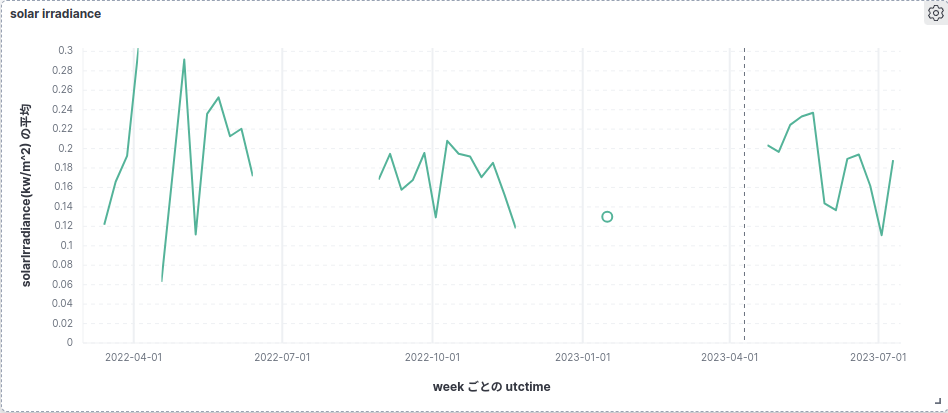
\includegraphics[width=160mm]{1.png}
    \caption{133.71.106.141のpcs\_recyclekan}
    \label{p1}
  \end{center}
\end{figure}

次に, 移行元である133.71.201.197のElasticSearchサーバーのpcs\_recyclekanインデックスに保存されたデータを図 \ref{p2}に示す.

\begin{figure}[H]
  \begin{center}
    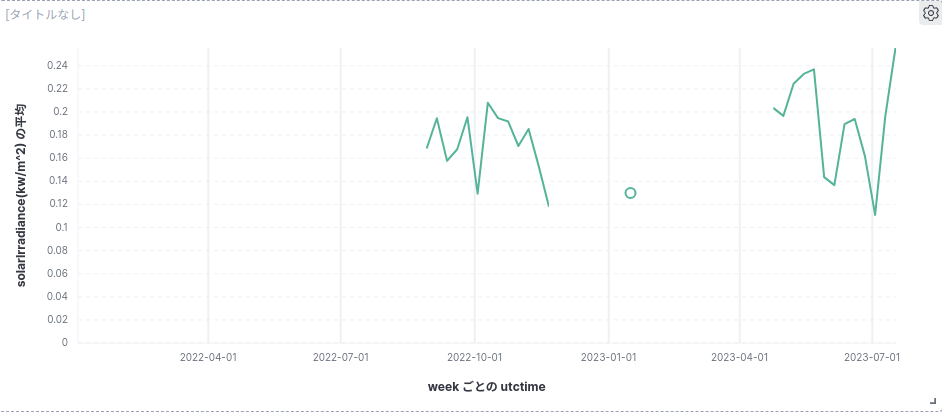
\includegraphics[width=160mm]{2.png}
    \caption{133.71.201.197のpcs\_recyclekan}
    \label{p2}
  \end{center}
\end{figure}

図 \ref{p1}, 図 \ref{p2}について, 2022年8月以降のグラフの概形が一致していることが確認出来るので, データ移行作業は正常に行うことが出来たと判断できる.

\section{movement\_diaryのデータについて}
movement\_diaryとmovement\_diary01はデータ型が異なる一部のフィールドを除いて全て同じデータを保有しており, それぞれのインデックスのドキュメント数の比較と, タイムスタンプ情報を格納するフィールドのインデックス間での比較を行うことで, movement\_diaryが不要なインデックスであるかを調査した.

まず, movement\_diaryとmovement\_diary01のドキュメント数を調べたところ, 同じ142件であった.

次に, movement\_diaryとmovement\_diary01でタイムスタンプ情報を持つフィールドであるdt\_Sフィールドの値同士を比較した.

ただし, dt\_Sフィールドがnullのドキュメントが一部存在するので, その場合はタイムスタンプ情報を持つinspectionフィールドの値同士を比較した.

比較した結果, dt\_Sフィールドとinspectionフィールドの両方がnullである3件のドキュメントを除いて他全てのドキュメントはdt\_Sフィールドもしくはinspectionフィールドの値がmovement\_diaryとmovement\_diary01の間で一致した.

dt\_Sフィールドとinspectionフィールドの両方がnullだった3件のドキュメントについても, 全てのフィールドにおいて, movement\_diary01のドキュメントがmovement\_diaryのドキュメントの持つ情報を持っていたので, これらの調査結果からmovement\_diaryインデックスはmovement\_diary01インデックスで代替でき, 削除して良いインデックスであると判断した.

\section{まとめ}
今回は, 133.71.201.197から133.71.106.141へのElasticSearchサーバー間のリサイクル館の太陽光パネルの測定データ移行とkibanaを用いた可視化結果について報告した.

移行元のデータと移行後のデータをkibanaで可視化して目視で比較したところ, 2022年8月以降のグラフの概形が一致していることが確認出来たので, データ移行作業は正常に行うことが出来たと判断できる.

また, 133.71.106.168のElasticSearchサーバーにあったmovement\_diaryインデックスとmovement\_diary01インデックスのドキュメントについて調査した結果を報告した.

調査結果より, movement\_diary01インデックスはmovement\_diaryインデックスの持つ全ての情報を保持しており, movement\_diaryインデックスは削除して良いインデックスであると判断した.

次回は, 133.71.201.197のElasticSearchサーバーにあるpcs\_recyclekanという名前のインデックス以外のインデックスについて調査を行い, 必要であればデータ移行を行う.

\begin{thebibliography}{5}
  \bibitem{1}Ferron H, ”ElasticDump”, https://github.com/elasticsearch-dump/elasticsearch-dump, 参照 June 19,2023.
\end{thebibliography}

\end{document}

